\chapter{书面翻译}

\title{从文件系统方面通过减少写入放大来延长基于闪存的存储的生命周期}

{\heiti 摘要:} 闪存由于其高性能,低能耗和低成本而作为用于企业和嵌入式系统的存储设备而广受欢迎。然而,闪存的耐用性问题仍然是一个挑战,随着存储密度随着多层单元(MLC)的采用而增加,这种问题正在变得越来越严重。之前的工作已经解决了损耗均衡和数据减少问题,但使用文件系统来提高闪存寿命的工作明显较少。传统文件系统中的一些常见机制(例如日志记录,元数据同步和页面对齐更新)会导致额外的写入操作并加剧闪存的磨损。这个问题被称为文件系统的写入放大。

为了减轻写入放大,我们提出了基于对象的闪存转换层设计(OFTL),其中的机制是与闪存协同设计的。通过利用页面元数据,OFTL能够实现索引元数据的惰性持久性,并在保持一致性的同时消除日志记录。粗粒度块状态维护减少了持久的空闲空间管理开销。借助字节单元访问接口,OFTL能够将小型更新与元数据进行压缩和共同定位,以进一步减少更新。实验表明,与最新页级别闪存转换层上的ext3,ext2和btrfs相比,基于OFTL的系统OFSS在SYNC模式下的写入放大率降低了47.4%〜89.4%,ASYNC模式下的写入放大率降低了19.8%〜64.0%。

\section{引言}
近年来,闪存技术有了很大的提高。随着主流设计从单层单元(SLC)转向多层/三层单元(MLC / TLC),基于闪存的存储正在见证容量的增加和每比特成本的降低,导致了在企业和嵌入式存储系统中应用的急速增长。但是,闪存密度的增加要求每个单元内有更精细的电压阶跃,这对泄漏和噪声干扰的耐受性较差。因此,闪存的可靠性和使用寿命大幅下降,产生了耐久问题[18,12,17]。

损耗均衡和数据缩减是延长闪存存储寿命的两种常用方法。通过磨损均衡,编程/擦除(P / E)操作倾向于分布在闪存块上,以使其均匀磨损[11,14]。数据缩减用于闪存转换层(FTL)和文件系统。 FTL引入了重复数据消除和压缩技术,以避免冗余数据的更新[15,33,34]。文件系统试图通过尾部打包[7]或数据压缩来减少更新[2,13]。但是,这些数据缩减技术在减少来自文件系统的写入放大方面效率低下,因为以下两个原因,从文件系统生成的元数据更新难以减少。一个是数据缩减不应损害文件系统机制。例如,在数据缩减中不应删除日志中的重复数据。另一个原因是大多数元数据出于一致性原因频繁同步,阻止了数据减少。

不幸的是,传统文件系统中的一些常见机制加剧了闪存写入放大。首先,通常用于保持更新原子化的日志记录加倍了写入大小,因为它将数据和元数据也复制到了日志。其次,元数据经常同步写入,以避免出现故障时的数据丢失。即使元数据占用的存储空间很小,频繁的写入操作也会产生巨大的写入流量,这对存储磨损产生巨大影响。第三,即使对于几个字节的更新,对存储设备的写入也是页对齐的。系统对来自应用程序的实际访问大小进行隐藏,因此更新强度被页面访问粒度放大。部分页面更新几乎总是需要读取 - 修改 - 写入。更糟糕的是,闪存页面大小的增加使得这个问题更加严重[17]。最后但并非最不重要的一点是,分层设计原则使得文件系统和设备彼此不透明,原因是窄块接口[35,29,28]。闪存存储上的文件系统机制无法解决耐久性问题,因此,使用这些机制,闪存会更快磨损。透明性还会阻止文件系统中的机制利用存储设备的特性。

事实上,闪存为更好的系统设计提供了机会。首先,每个页面都有一个页面元数据区域,也是OOB(带外)区域。保留空间可用于为索引元数据的惰性持久性或提供写入原子性的事务信息保留反向索引。其次,块被擦除后,闪存块的全部区域都变为干净状态。可以通过以擦除块(256 KB)为单位跟踪空闲空间而不是文件系统块(4 KB)来减少元数据开销。第三,与HDD(硬盘驱动器)相比,随机读取性能显著提高。部分页面更新可以被压缩,而不会引入显着的随机读取惩罚。如上所述,闪存特性可以用来缓解与系统协作时的耐久性问题。

我们提出了一种名为OFTL的基于对象的闪存转换层设计,将存储管理卸载到对象存储,并与闪存共同设计系统以减少写入放大。我们的贡献总结如下:

\begin{itemize}
\item 我们提出了OFTL,一个基于对象的闪存翻译层,以促进对数据的组织方式进行语义感知。
\item 为了降低索引元数据持久性和日志记录的成本,我们懒惰地刷新索引并通过在页面元数据中保留反向索引和事务信息来消除日志记录。
\item 我们还使用粗粒度块状态维护来跟踪页面状态,以降低可用空间管理的成本。
\item 使用OFTL中的字节单元接口,我们压缩部分页面更新并将它们与元数据共同定位以减少页面更新次数。
\item 我们实施基于OFTL的系统并在不同类型的工作负载下对其进行评估。结果显示,与现有文件系统相比,写入放大率显着降低。
\end{itemize}

本文的其余部分安排如下。第2部分给出了闪存和基于闪存的存储系统体系结构的背景。然后,我们在第3部分中介绍我们的OFTL设计,并在第4部分中与闪存共同设计系统机制。我们在第5部分中描述了实现,并在第6部分中评估了设计。相关工作在第7部分中介绍,第8节给出了结论。

\section{背景}
\subsection{闪存基础}
闪存以页为单位读取或写入,并以闪存块单位擦除。页面大小范围从512B到16KB [11,17]。每个Flash页面都有页面元数据,这些页面元数据与页面数据一起自动访问。通常,一个4KB页面有128B页面元数据[11]。闪存块由闪存页面组成,例如,一个256KB闪存块包含64页[11]。闪存块进一步排列在平面和通道中,以便在闪存驱动器内进行并行处理,称为内部并行。

与硬盘驱动器相比,闪存具有两个独特的特征,即不可覆盖属性和耐久性限制,这些都应该被文件系统设计考虑到。不可覆盖属性意味着被编程的页面不能被重新编程,直到它所在的闪存块被擦除。对编程页面的更新被重定向,以不可覆盖的方式清除页面,而编程页面无效以后再擦除。耐久性限制是每个存储器单元具有有限数量的P / E操作。存储器单元耗尽更多的P / E周期,导致寿命和可靠性的恶化。

\subsection{基于闪存的存储系统的体系结构}
闪存在嵌入式系统中广泛使用。在嵌入式系统中,闪存不支持块接口,并由文件系统直接管理,在该系统中实现映射,垃圾收集和耗损均衡。文件系统专用于闪存,称为闪存文件系统[10,32],如图1(a)所示。随着容量的增加和成本的降低,从笔记本电脑到企业服务器的计算机系统采用闪存设备作为HDD的替代品。 FTL在设备固件中实现以提供块接口,如图1(b)所示。

由于嵌入式FTL需要来自嵌入式处理器和大型DRAM的巨大计算能力来增加设备容量,因此FusionIO在称为VSL(虚拟存储层)的软件中实现了FTL,共享主机CPU周期和主存储器容量[4]。图1(c)显示了架构。基于软件的VSL为文件系统提供了优化的机会。在VSL上提出了DFS以利用VSL中的存储管理[20],并且使用日志结构的FTL从VSL中导出原子写入接口以向系统提供写入原子性[28]。

\begin{figure}[h]
  \centering
  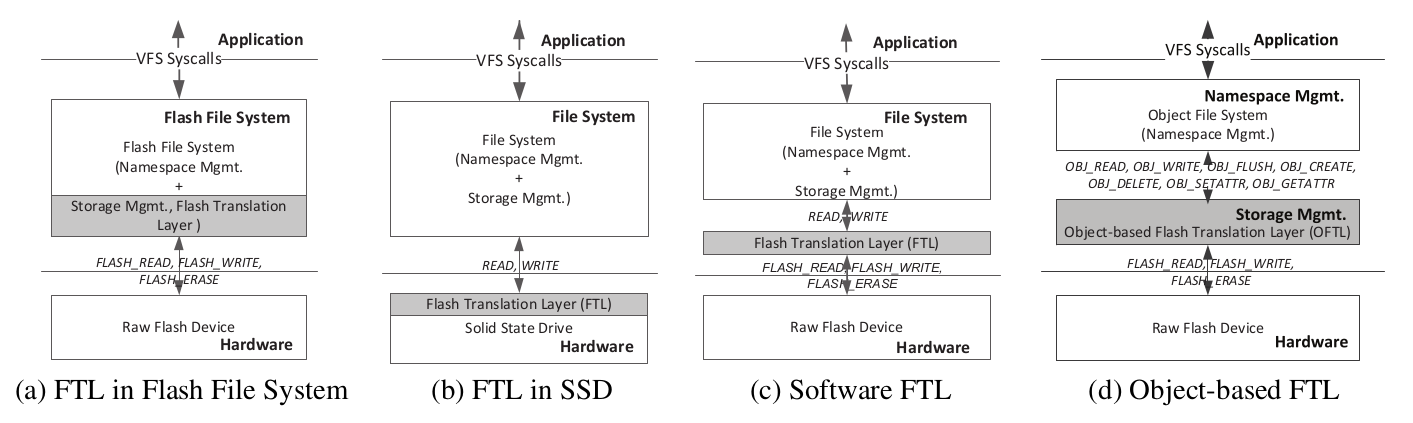
\includegraphics[width=0.8\textwidth]{translate_fig1.png}
  \caption*{图~1\hskip1em 基于闪存的文件系统结构}
\end{figure}

尽管基于软件的FTL比嵌入式FTL具有更好的性能,但文件系统和FTL之间的窄块接口阻止文件系统或FTL的优化。文件语义隐藏在狭窄的界面之后,阻碍了智能存储管理[35,26]。此外,闪存属性对文件系统不透明,导致文件系统优化失去了机会[20,29,28]。与基于对象的SCM [21]类似,我们提出了基于对象的FTL设计OFTL,以便与文件系统和闪存更好地配合,如图1(d)所示。在基于OFTL的体系结构中,存储管理从文件系统移动到OFTL以直接管理闪存,因此可以调查闪存属性以优化文件系统机制设计,如元数据同步的日志删除和频率降低。 OFTL通过读/写/擦除操作管理闪存,并直接访问每个闪存页面的页面元数据。另外,OFTL将字节单位访问接口导出到文件系统,这是一个基于对象的文件系统,不受存储管理的限制,只能管理名称空间。

\section{基于对象的闪存转换层}
基于OFTL的体系结构将存储空间管理从文件系统卸载到OFTL,以更好地协同设计文件系统和FTL。 OFTL访问页面单元接口中的原始闪存设备,同时将字节单元访问接口导出到文件系统。因此,OFTL将从每个对象的逻辑偏移量映射到Flash页面地址。在本节中,我们将描述OFTL接口和数据组织。

\begin{table}[htb]
    \centering
    \begin{minipage}[t]{0.8\linewidth}
    \caption*{表~1\hskip1em 对象接口}
      \begin{tabularx}{\linewidth}{lX}
        \toprule[1.5pt]
        {\heiti 操作} & {\heiti 描述} \\\midrule[1pt]
        \textbf{oread}(devid, oid, offset, len, buf) & 从编号为oid的对象的offset位置读取数据到buf\\
        \textbf{owrite}(devid, oid, offset, len, buf) & 向编号为oid的对象的offset位置写入buf中的数据\\
        \textbf{oflush}(devid, oid) & 将编号为oid的对象的数据和元数据持久化\\
        \textbf{ocreate}(devid, oid) & 创建编号为oid的对象\\
        \textbf{odelete}(devid, oid) & 删除编号为oid的对象\\
        \textbf{ogetattr}(devid, oid, buf) & 获取编号为oid的对象的标签\\
        \textbf{osetattr}(devid, oid, buf) & 设置编号为oid的对象的标签\\
        \bottomrule[1.5pt]
    \end{tabularx}
\end{minipage}
\end{table}

{\heiti OFTL接口。} OFTL将字节单位读/写接口导出到文件系统,以直接将访问大小以字节为单位传递给OFTL。表1显示了对象接口。 oread和owrite接口都将字节单位的偏移和len传递给OFTL,而不是扇区单元。因此,OFTL从应用程序中获得准确的访问大小,从而可以将小更新压缩成更少的页面,这在4.3节中讨论。另外,使用对象接口中提供的oid对每个对象进行操作,这使得OFTL知道所访问页面的数据类型。 OFTL利用对象语义对更新关联数据进行聚类。此外,OFTL使用类型语义区分数据页面的索引页面,以便在页面元数据中保留辅助元数据以实现懒惰索引,这在4.1节中讨论。
OFTL以页面单元读取/写入操作和块单位擦除操作访问闪存。页面元数据读/写可以在NVMe规范[6]之后直接从OFTL访问,该规范定义了用于访问PCI Express总线上的非易失性存储器的主机控制器接口。

\begin{figure}[h]
    \centering
    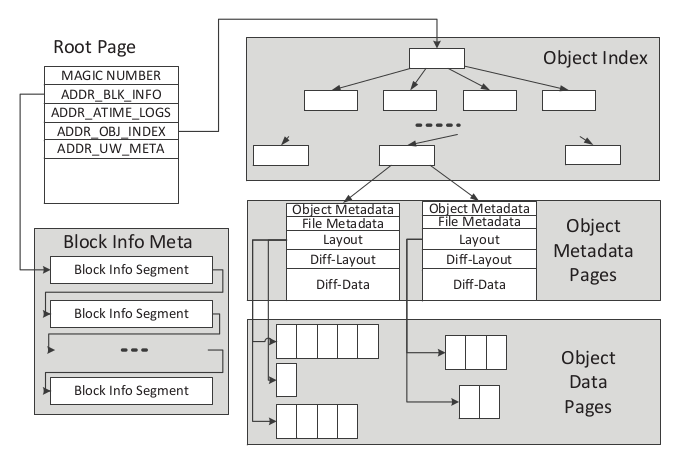
\includegraphics[width=0.8\textwidth]{translate_fig2.png}
    \caption*{图~2\hskip1em OFTL结构}
  \end{figure}

{\heiti 数据组织。 } OFTL由两个主要部分组成,对象存储和块信息元数据。单个根页面标识每个对象存储和块信息元数据的位置,如图2所示。对象存储分为三个级别:对象索引,对象元数据页面和对象数据页面。对象索引使用B +树将对象ID映射到其对象元数据。对象元数据包含传统上存储在文件系统索引节点中的信息,包括引用对象数据页面中的地址的分配信息。
块信息元数据保持每个闪存块的元数据信息,包括闪存块状态,无效页数(其数据过时但未被擦除)以及每个闪存块的擦除次数。每个闪存块有三种状态:FREE,UPDATING和USED,每个页面有三种状态:FREE,VALID和INVALID,这些在第4.2节中有解释。块信息元数据是以日志结构化的方式编写的。每个块信息条目有32位,其中20位用于擦除计数,10位用于无效页数,2位用于闪存块状态。块信息不是与每个闪存块一起存储,而是存储在闪存中的一个单独的空间中,这会在垃圾收集期间导致更少的页面更新。

\section{系统与闪存的协同设计}
OTFL使用三种技术来利用底层闪存设备的特性。在4.1节中,我们介绍了Backpointer-Assisted Lazy Indexing,这是一种有效维护数据和元数据之间一致性的机制。在4.2节中,我们介绍了我们的粗粒度块状态管理方法,它可以降低状态写入的频率。在第4.3节中,我们介绍了我们的压缩更新技术,该技术摊分了跨多个未对齐页面写入的页面写入成本。

\begin{figure}[h]
    \centering
    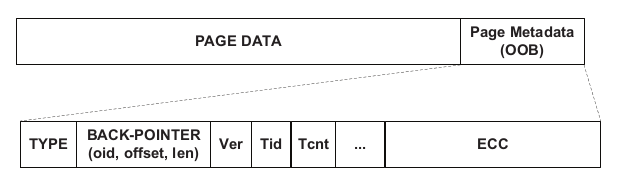
\includegraphics[width=0.8\textwidth]{translate_fig3.png}
    \caption*{图~3\hskip1em 页元数据}
  \end{figure}

\subsection{反向指针辅助的惰性索引}
索引元数据(对象元数据页面中用于指向数据页面的数据布局的指针或者指向对象索引以指向对象元数据页面的指针)应该同步写入以防存储设备损失或不一致。索引元数据的同步也称为索引持久性。虽然典型指针的大小为8个字节,但索引持久性会更新整个页面,即4KB或更大。因此,频繁的索引持久性导致严重的写入放大。

在索引元数据的惰性持久性中,在每个索引页面的页面元数据中采用了类型特定的反向指针技术,以减少索引持久化的频率,同时保持一致性。如图2所示,对象索引,对象元数据页面和对象数据页面在树结构中进行索引并形成三级分层结构。图3说明了页面元数据组织。在OFTL中,我们有两种类型的后向指示器(oid,offset,len)。一个用于数据页面来对对象元数据进行逆向索引,oid和offset,len分别表示对象id,对象中的逻辑页面偏移量和页面的有效数据长度。另一个用于对象元数据页面来反向索引对象索引,并且只有oid被设置为表示对象ID。在写入反指针时,首先设置类型以指示反指数的类型,以便可以针对不同类型正确理解反指针。我们也保留版本以确定最新的恢复页面版本。因此,类型特定的反向指针用作反向索引,并且索引持久化与页面更新解耦。

为了减少反向索引的扫描时间以在系统故障后重建索引元数据,我们使用更新窗口来跟踪最近分配的未完成索引元数据持久化的闪存块。更新窗口由检查点进程维护,检查点进程在更新窗口中的空闲页数低于阈值并且需要扩展窗口时触发。更新窗口描述了在发生故障后需要检查其反向索引的块集,因为索引可能不会引用它们。

更新窗口还提供多个页面的更新原子性。页面元数据保存事务信息(tid,tcnt),其中tid是每个写入操作的更新窗口中的唯一ID,tcnt是更新中页面的数量。对于写操作的所有页面,只有一个页面具有tcnt设置,其他页面的tcnt值为零。 tcnt用于在系统故障后检查操作的完整性。垃圾收集不允许在更新窗口中的闪存块上执行,以便完成原子性检查的事务信息。因此,使用闪存提供的写入原子可以消除日志。

在系统故障后重新启动时,扫描更新窗口中的对象数据页面。首先检查交易信息以确定涉及该页面的写入操作的完整性。如果写入不完整,则写入的所有页面都将被丢弃。这样就保证了原子性。在检查之后,如果在系统失败之前对象布局未被写入稳定,则读出后向指针以更新对象布局。由于所有更新都位于自上次检查点以来的更新窗口中,因此可以通过从当前更新窗口重新构建扫描页面中的后向指示器,将对象布局更新为最新版本。文件大小元数据也会随着所有有效数据大小的重新计算而更新。虽然其他描述性元数据(如修改时间和访问控制列表)在意外崩溃后可能会丢失,但系统一致性不会受到影响。类似地,可以用对象元数据页面的当前更新窗口的扫描来更新对象索引。通过页面元数据和更新窗口中的辅助信息,可以减少索引持久化频率,并提供写入原子性来消除日志。

\begin{figure}[h]
    \centering
    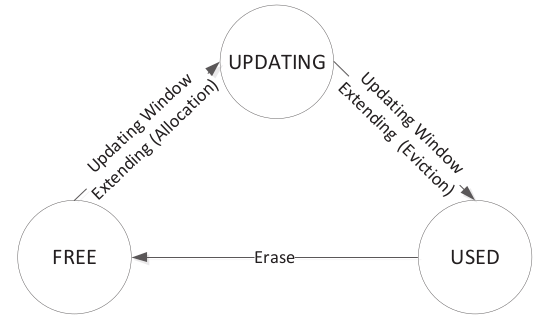
\includegraphics[width=0.8\textwidth]{translate_fig4.png}
    \caption*{图~4\hskip1em 闪存块的状态转换}
  \end{figure}

{\heiti 一致性和耐久性讨论。} 在懒惰索引技术中,系统崩溃后,除索引指针和大小之外的元数据可能会丢失。 这导致元数据的过时版本,这伤害元数据更新的持久性。 与耐久性相比,我们将一致性视为更重要的事情,因为索引的腐败会导致文件系统的不一致甚至失败。 我们使用懒惰索引技术来保证索引和大小可以在恢复期间重建。 但是对于持久性问题,我们选择让文件系统或应用程序确定让其他元数据持久化的时间,并显式同步。

\subsection{粗粒度块状态维护}
在闪存中,每个页面都有三种状态:FREE,VALID和INVALID。空闲页面是尚未写入的页面。有效页面是已写入的页面,其数据是有效数据。无效页面是已写入但其数据已过时的页面。有效和无效页面也称为INUSE页面。每个闪存块也有三种状态:FREE,UPDATING和USED。空闲块中的页面全部为空闲页面,已使用块中的页面全部处于使用页面中,而只有更新块同时具有空闲页面或未使用页面。由于页面是按顺序写入闪存块中的,因此最新分配的页码用于将空闲页面与更新块的使用中分开。因此,OFTL通过跟踪闪存块状态来区分空闲页面和使用中页面。对于inuse页面,索引元数据用于进一步区分有效页面和无效页面。有效页面在索引元数据中编入索引,而无效则不在索引中。因此,可以通过跟踪闪存块的状态来识别空闲,有效的无效页面,并且通过闪存块单元中的状态维护而不是页面单元来减少空闲空间管理成本。

OFTL通过降低元数据持久性的频率来进一步降低成本。闪存块状态的持久性仅在闪存块被分配给或从更新窗口驱逐出时执行,如图4的顶部所示。状态持久性被放宽,但是满足以下两个条件:(1)持久性空闲块是实际空闲块集的子集; (2)持续无效页面的数量不超过无效页面的实际数量。

第一个条件意味着一个空闲块可以被认为是非空闲的,这可能导致分配丢失。但是一个非空闲块不能被视为空闲,否则写入失败。它要求从FREE到UPDATING的状态转换立即刷新,但将状态持久性从USED释放到FREE。第二个条件放松了无效页面的数量持久性。无效页面的数量用于选择驱逐的闪存块并检查垃圾回收期间移动的有效页面的数量。通过检查索引元数据来区分有效页面和无效页面。在达到有效页面的数量之前,剩余的所有页面都是无效的,并且不再需要无效的页面检查,从而使被驱逐块的页面移动停止。在最坏的情况下,如果无效页面的持续数量少于实际数量,则必须检查所有页面。由于系统崩溃很少出现,所以对垃圾收集效率的影响是有限的。类似于无效页面的持续数量,记录的擦除次数可能会保持不变,这也可以接受,因为擦除次数不敏感。

总之,空闲空间管理从粗粒度块状态维护中受益,因为闪存块粒度状态跟踪和状态持久性的降低都减少了元数据成本。

\subsection{压缩更新}
通过字节单元访问接口,OFTL能够识别部分页面更新,这些页面更新只更新一页的一部分,既适用于小于一页的小型更新,也适用于大型更新的正面/反面。压缩更新技术压缩同一对象的部分页面更新,并将它们与其对象元数据页面共同定位以减少更新页面。

\begin{figure}[h]
    \centering
    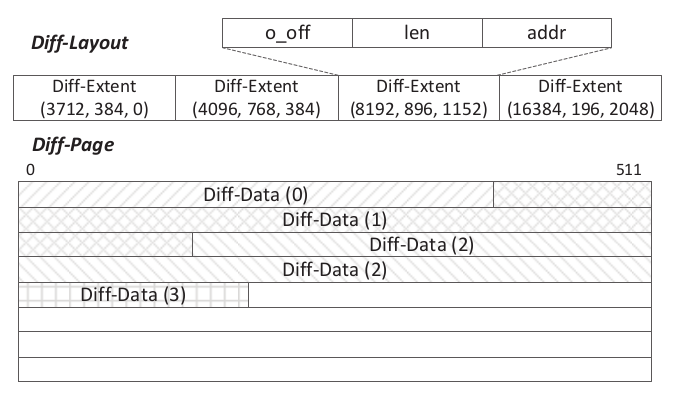
\includegraphics[width=0.8\textwidth]{translate_fig5.png}
    \caption*{图~5\hskip1em Differential Layout(Diff-Layout)数据结构}
  \end{figure}

{\heiti 部分页面更新。} OFTL中的部分页面更新被压缩并插入差异页面,又名差异页面。存储在diff-page中的每个数据段都称为diff-data。 Diff-data使用三元组<ooff,len,addr>进行diff-extent索引,其中ooff和len分别表示对象偏移量和diffdata的长度,addr是diff-数据在diff-页。 Diff-extents在diff-layout中按照对象偏移量的升序保持不变。每个对象都有一个diff-layout,它是一个对象的所有diff-extents的集合。图5显示了数据结构。

尽管部分页面更新被吸收到差异页面中,而差异页面在差异布局中编入索引,但整个页面更新会直接写入对象页面。对象页面在布局中进行索引,这是一个对象的所有范围的集合,用于保存完整页面的起始地址和长度对。与差异布局一样,布局也记录在对象元数据页面中,如图2所示。在压缩更新技术中,读取,写入和合并操作如下所述:

\begin{itemize}
    \item 写入:写入数据分为多页。不开始或结束页面对齐的部分被标识为部分页面更新,而其他部分则被认定为整页更新。然后部分页面更新在diff-pages中更新。因为部分更新总是取代整个页面,所以整个页面更新必须使相应的差异数据无效并删除其差异范围,然后更新布局以引用整个页面。
    \item 合并:当差异页面已满时需要合并操作。合并时,会扫描diff-extents以选择在diff-pages中消耗最多空间的驱逐的逻辑页面。然后读取驱逐的逻辑页面的对象页面并与diff-data合并。之后,合并的页面被写入新的对象页面,并且相应的diff-data和diff-extents被删除。
    \item 读取:首先以不同的格式检查读取操作。如果它在diff-data中被满足,则读缓冲区被diff-data填充。否则,读取对象页面并与任何现有的对应diff-data合并。
\end{itemize}

{\heiti 更新协同定位。} 在大多数情况下,每个对象的元数据大小远小于页面大小。 OFTL不是压缩多个对象的元数据,而是与对象元数据页面不同的页面。 由于每个数据更新之后都有元数据更新,例如文件大小或修改时间,因此diff-data和元数据页面的共同位置通常会节省一页写入。 在协同定位中,diff-page的大小小于一个页面大小,并且取决于对象元数据的大小更改。 diff-page的大小是通过从flash页面大小中减去元数据大小来计算的,flash页面大小用于检查diff-page是否已满。 一旦完成,触发合并操作以选择一些diffdata并将它们合并到对象数据页面。 通过这种方式,部分页面更新的成本通过压缩和协同定位来分摊。

\section{实现}
我们在Linux内核3.2.9中实现OFTL作为内核模块。该模块由三层组成:转换层,缓存层和存储层。

转换层遵循图2所示的设计。使用Log-Structured Merge Tree(LSM-Tree)[27]实现闪存对象索引,该索引具有用于快速查找的内存B +树并添加记录每个对象索引更新的<operation,object ID,phy addr>。每个对象都有一个内存中对象的元数据数据结构,它记录访问统计信息和两个基于范围的布局,以及图2所示的闪存对象元数据页面。diff-layout和layout都链接它们的范围在内存中的列表结构中。在写入请求上,写入数据首先分页对齐。整页更新被写入数据页面,然后进行布局更新,而部分页面更新被插入diff-data,然后是diff-layout更新。对象操作转换为元数据或数据页面上的读/写操作并转发到缓存层。

元数据和数据页面缓存在缓存层中。 OFTL缓存遵循linux内核中页面缓冲区的设计,不同之处在于替换是用整个对象完成的。在写操作时,如果设置了SYNC标志,则高速缓存检查SYNC标志并从存储层调用闪存写入接口。否则,更新缓存层中的对象缓存。页面分配被延迟直到页面需要刷新。然后,缓存层从更新窗口分配空闲页面并调用闪存写入接口以通过存储层写入页面。

存储层从缓存层接收闪存读/写/擦除操作,构建bio请求,并将它们发送到通用块层。我们使用系统中的TRIM / DISCARD命令和SATA协议来执行擦除操作。 OOB的DMA传输遵循NVMe标准中的设计[6]。由于硬件限制,目前在存储器中模拟OOB操作。

\begin{figure}[h]
    \centering
    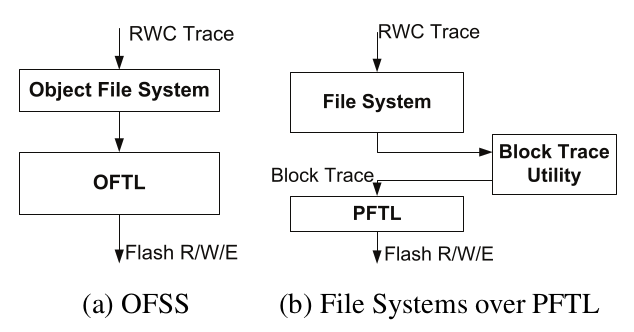
\includegraphics[width=0.8\textwidth]{translate_fig6.png}
    \caption*{图~6\hskip1em Trace驱动的模拟框架}
  \end{figure}

在OFTL中,我们使用简单的垃圾收集和磨损平衡策略。当空闲块的百分比下降到15%以下时开始垃圾收集,并一直持续到百分比超过该值。在耗损均衡中,擦除次数的上限用于防止闪存块擦除次数过多。在平均擦除次数增加后,这一上限会周期性地上升。我们将在未来纳入更好的战略。

为了评估其他文件系统解决方案,我们还实现了一个简单的目标文件系统来解析命名空间,如图1(d)所示。目标文件系统使用内存中的哈希表来保持从路径到对象ID的映射,并通过将对象ID替换为路径将IO请求传递给OFTL。我们在评估部分调用基于OFTL的系统对象闪存存储系统(OFSS)。

\section{评估}
我们测量写入放大率,写入闪存的总大小/计数,除以应用程序发出的写入总大小/计数,以评估OFSS的写入效率以及ext3,ext2和btrfs最新的页面级FTL。

在本节中,我们首先评估这四个系统的总体性能,然后分析元数据放大。我们还测量闪存页面大小的影响以及扩展OFTL设计带来的更新窗口的开销。

\begin{table}[htb]
    \centering
    \begin{minipage}[t]{0.8\linewidth}
    \caption*{表~2\hskip1em 工作负载特性}
      \begin{tabularx}{\linewidth}{lXXXX}
        \toprule[1.5pt]
        {\heiti 负载名称} & {\heiti 写次数} & {\heiti 写大小(KB)} & {\heiti 刷新次数} & {\heiti 不对齐写的百分比} \\\midrule[1pt]
        iPhoto & 496542 & 6651962 & 37054 & 51.2\%\\
        iPages & 75661 & 183728 & 565 & 99.6\%\\
        LASR-1 & 32249 & 42600 & 1714 & 93.3\%\\
        LASR-2 & 111531 & 216114 & 14998 & 99.0\%\\
        LASR-3 & 21956 & 24426 & 3056 & 96.1\%\\
        TPC-C & 26144 & 219689 & 489 & 7.1\%\\
        \bottomrule[1.5pt]
    \end{tabularx}
\end{minipage}
\end{table}

\subsection{实验设置}
我们从系统级IO跟踪中提取读取,写入和关闭操作(RWC跟踪)并在文件系统和OFSS上重放它们。图6显示了tracedriven仿真框架。在重放程序中,关闭操作会在文件系统中执行fsync操作或在OFSS中执行对象刷新操作。在OFSS中,我们将I / O的数量和大小收集到OFTL存储层的闪存中。在文件系统评估中,我们使用blktrace实用程序[1]在文件系统评估中捕获存储设备上的I / O,然后在PFTL上重播块跟踪,PFTL是在Linux kernel-3.2中作为内核模块实现的模拟页级FTL。 9。我们收集PFTL中闪存的I / O数量和大小。在仿真中,PFTL使用类似于主存储器管理的两级页表将逻辑页号转换为物理页号。 LazyFLT [23]功能集成到PFTL中以减少映射开销。

我们评估桌面环境中iBench [19]的两个工作负载,服务器环境中LASR [5]的三个一个月跟踪以及数据库管理系统中的一个TPCC跟踪。 TPC-C跟踪是使用strace实用程序[8]从运行在PostgreSQL上的DBT2工作负载[3]收集的。表2列出了六项工作量的特点。

实验在SUSE Linux 11.1上进行,Linux内核3.2.9在4核Intel Xeon X5472 3GHz处理器和8GB内存的计算机上运行。除用于操作系统的磁盘驱动器外,还使用Seagate 7200rpm ST31000524AS磁盘驱动器进行跟踪收集。在实验中,ext3和ext2使用noatime,nodiratime选项进行挂载,而btrfs使用ssd,discard和lzo选项进行挂载。在OFSS设置中,默认页面大小为4KB,闪存块大小为256KB。对象数据和元数据的更新窗口都设置为64个闪存块的大小。默认的OFTL缓存大小为32MB。

\subsection{总体比较}

\begin{figure}[h]
    \centering
    \caption*{表~3\hskip1em 写放大的整体评估}
    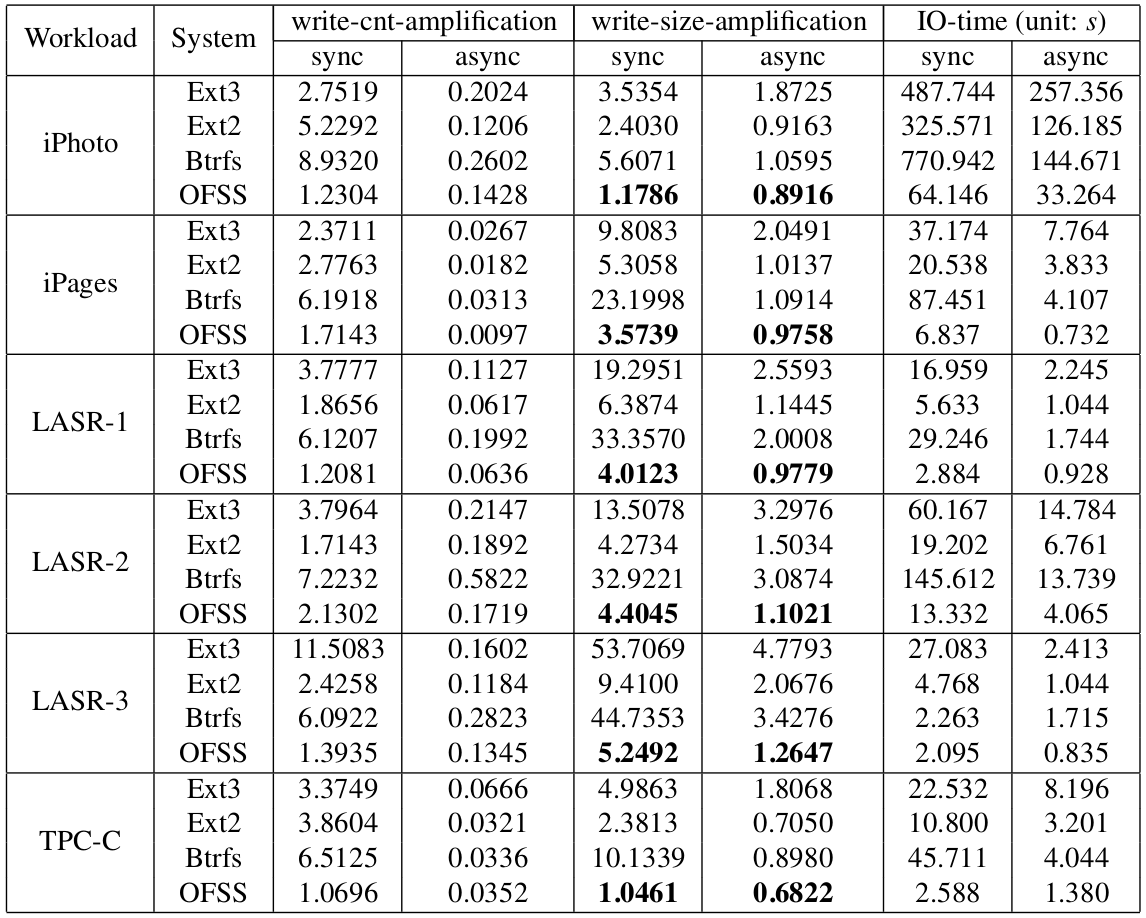
\includegraphics[width=0.8\textwidth]{translate_tab3.png}
  \end{figure}

在本节中,针对建立在PFTL上的ext2,ext3和btrfs,针对OFSS评估写入效率和IO时间。为了提供数据一致性,ext3使用数据日志选项装载,而btrfs使用写入时复制来更新数据,而ext2则不提供一致性。 OFSS通过利用闪存的不覆盖属性并将事务信息保存在页面元数据中来提供数据一致性。这四个系统以SYNC和ASYNC模式进行评估。在SYNC模式下,数据和元数据在请求返回之前需要刷新稳定。 Ext2和ext3使用同步选项安装以支持SYNC模式。 Btrfs在文件打开操作中使用O SY NC标志,因为btrfs中不支持sync安装选项。在ASYNC模式下,数据和元数据被缓存在内存中,直到显式同步,时间到期或缓存逐出。三个文件系统的默认挂载选项支持ASYNC模式。

表3显示了在SYNC模式下每个系统的总写入次数和写入大小所测得的写入放大倍数。写入计数在ext3,ext2,btrfs和OFSS中的平均写入放大倍数分别为4.60,2.98,6.85和1.11。写入大小的写入放大显示类似的结果,并且ext3,ext2,btrfs和OFSS中的平均值分别为17.47,5.03,24.99和2.64。差异主要来自与写入操作相关的元数据成本。在ext2中,写操作具有数据更新,inode更新的子操作,并且如果需要空间分配,则有时会更新位图。在使用数据日志的ext3中,数据和元数据复制到日志日志中,然后进行提交/异常同步写入,稍后通过日志守护进程对实际位置进行检查点设置。即使写入计数在ext3和ext2中由于合并写入而在检查点中接近,由于在日志日志中添加了重复的数据和元数据,ext3中的写入大小仍然远远大于ext2中的写入大小。在SYNC模式下,btrfs将更新记录到特殊的日志树中以消除整个系统更新[30],从而导致写入放大率高。 Btrfs针对性能进行了优化,它使用“ssd”分配方案进行免寻找分配,并且尚未针对闪存耐久性进行优化[2]。随着杂志的淘汰,元数据同步频率的降低和压缩更新,OFSS相对于其他三种传统文件系统的写入放大率降低了47.4%〜89.4%。

如表3所示,ASYNC模式下的写入放大率分别为0.13,0.09,0.23和0.09,写入次数分别为2.73,1.23,1.93和0.98,写入大小分别为ext3,ext2,btrfs和OFSS。在ASYNC模式下,写入放大并不像SYNC模式那样糟糕。原因是元数据同步不频繁,元数据更新在缓冲区以及数据中合并。但是,由于日志记录,ext3中的写入强度加倍。 Btrfs必须更新用于写入时复制更新机制的索引元数据,消耗更多页面。此外,当页面未对齐时,页面对齐的更新机制会浪费空间,这会对所有三个传统文件系统产生写入放大效果。相比之下,与三个传统文件系统相比,OFSS性能更好,写入放大率降低了19.8%〜64.0%。

总体IO时间也显示在表3中以进行性能比较。由于硬件限制,我们通过向SSD发出请求而不是原始闪存来评估性能。由于我们设计的重点是写入放大减少而非映射策略的性能导向设计,垃圾收集或耗损均衡,因此SSD内部的FTL对性能评估影响不大。我们收集和累积每次操作的设备I / O时间,这是从操作到SSD的问题到SSD的确认的度量。如图所示,两种模式下的OFSS性能都明显优于其他模式。写入大小的减少不仅延长了闪存存储的使用寿命,而且还提高了性能。此外,性能改进部分来自基于对象的FTL设计,该设计使用OFTL缓存中的延迟空间分配来实现更好的I / O调度。

{\heiti 工作量讨论。} 一般而言,OFSS为拥有大量页面未对齐更新或频繁数据同步的工作负载带来更大的好处。当同步写入操作时,传统文件系统需要多个页面,包括数据,inode和位图文件系统块的页面才能更新。元数据开销对小更新很重要,其中只更新了几个字节。平均更新大小小于1KB的LASR-1和LASR3工作负载在SYNC模式下暴露了无法接受的写入放大,而OFSS极大地减少了元数据开销,并且使得放大率更低。由于压缩更新技术,未对齐的页面更新也可以从OFSS中受益。一个反例是TPC-C工作负载,它在用户空间中拥有自己的缓冲区,并以页为单位写入数据。 OFSS对TPC-C工作负载的改进不如其他工作负载那么重要。

\subsection{元数据的写放大}

\begin{figure}[h]
    \centering
    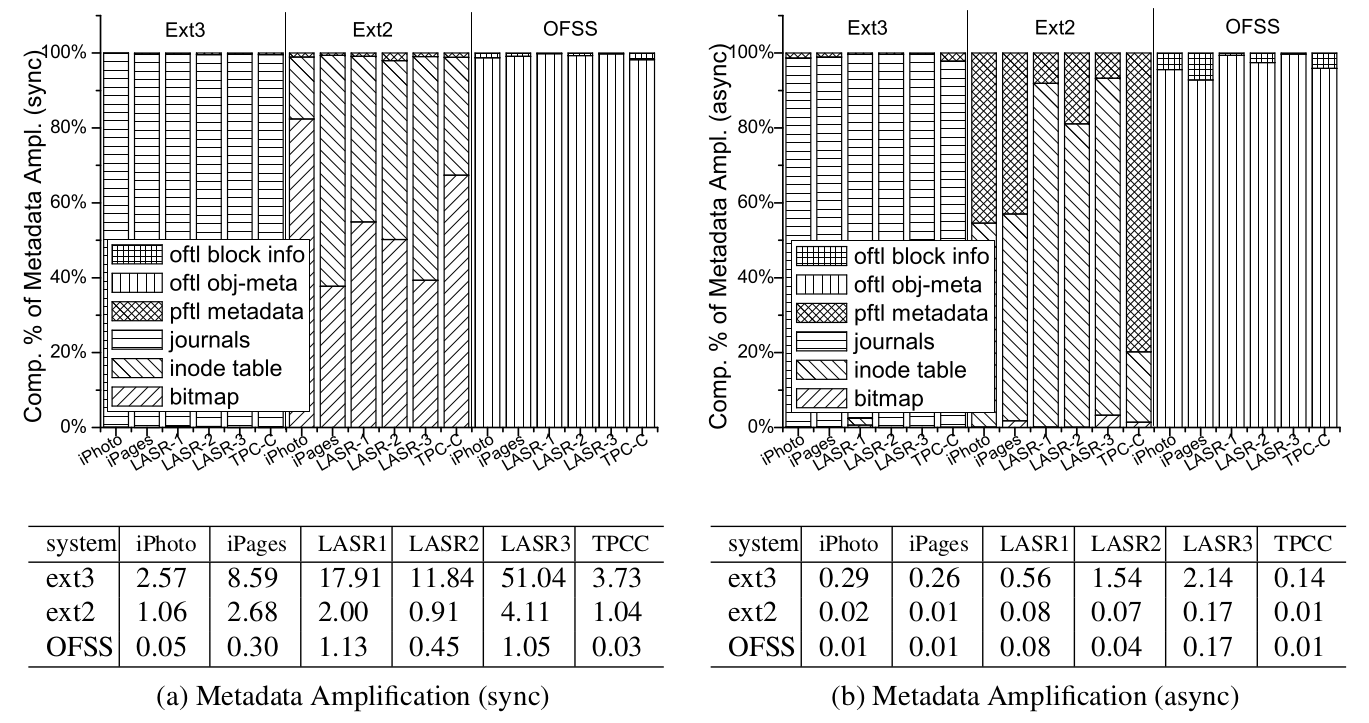
\includegraphics[width=0.8\textwidth]{translate_fig7.png}
    \caption*{图~7\hskip1em 元数据的写放大}
  \end{figure}

为了进一步了解OFSS的改进以及期刊移除和元数据同步缩减的效果,我们仔细研究元数据放大。在评估中,我们通过使用dump2 f s命令的转储信息检查ext2和ext3的物理布局来识别每个访问的文件系统块类型。日志类型由块跟踪中的“k日志”标识。我们从此分析中忽略了btrfs,因为我们无法区分块跟踪中写入地址的元数据和数据更新。图7显示了表格中的总元数据放大率以及SYNC和ASYNC模式中表格上方的各种元数据的百分比。

从图7中,ext3的元数据放大有两个观察。一个是与文件系统元数据的写入放大相比,PFTL的写入放大可以忽略不计。另一个原因是日志显着地放大了写入并且控制了成本。 ext2和ext3之间的区别验证了日志删除的好处。在下文中,我们将通过将OFSS与ext2进行比较来进一步了解减少元数据同步的好处。

在元数据同步减少评估中,我们在计算OFTL的元数据放大时,从OFSS中的元数据页面中去除差异数据。如图7(a)所示,inode和bitmap更新消耗了SYNC模式中大部分的放大。 inode更新的写入放大率从平均值ext2中的0.99降至OFTL元数据更新所测量的OFSS中的0.50。好处不仅来自懒惰索引,而且来自使用压缩更新的已摊销元数据页更新成本。文件系统块位图更新的写入放大率从平均ext2中的0.93降低到用OFTL闪存块信息更新测量的OFSS中的0.0019,其显示了粗粒度块状态维护的益处。由于空闲空间是以闪存块单位进行管理的,实验中为64页(256KB),比ext2中的4KB块大得多,因此粗粒度块状态维护极大地有利于自由空间管理。

在如图7(b)所示的ASYNC模式下,inode和元数据更新成本分别是ext2和OFSS的主要成本。他们两人的写入放大成本平均在0.05左右。传统文件系统将多个inode压缩到一个inode表文件系统块中,与OFSS中的压缩更新技术相比,这是一种减少元数据放大的不同方法。这两种方法在ASYNC模式下都有类似的效果。 ext2中的文件系统块位图在ASYNC模式下进行缓存和合并,使成本接近OFSS中的闪存块状态维护成本。

\subsection{闪存页面大小的影响}

\begin{figure}[h]
    \centering
    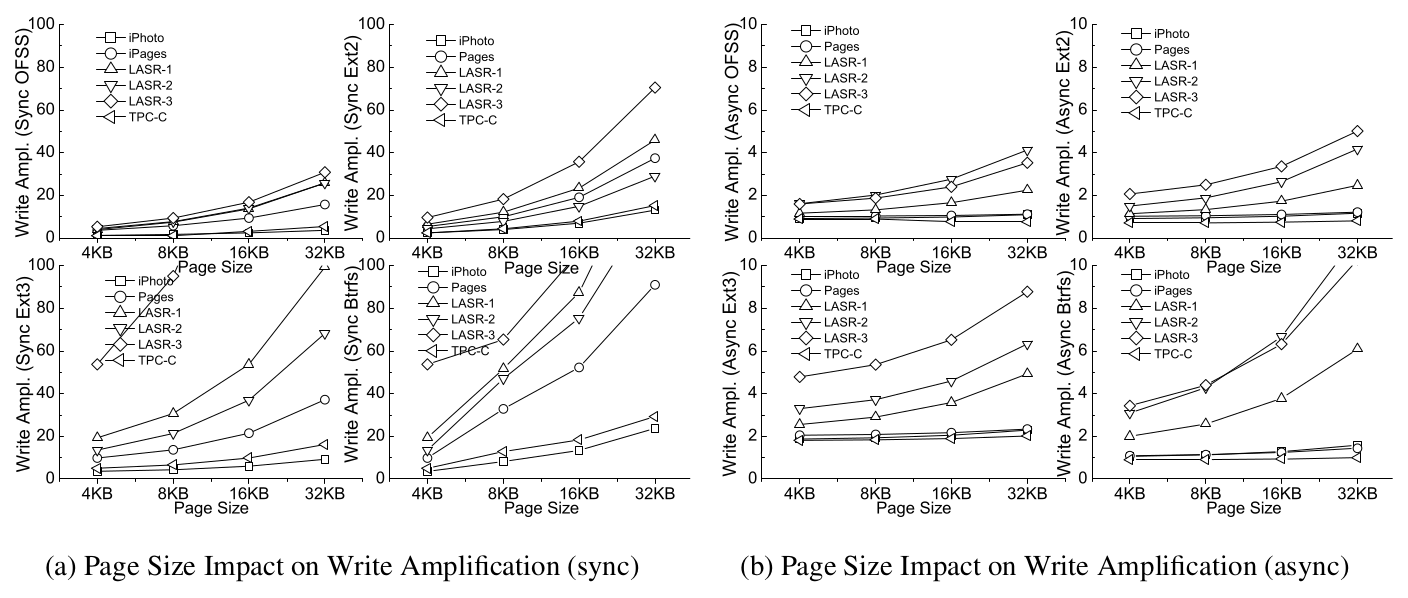
\includegraphics[width=0.8\textwidth]{translate_fig8.png}
    \caption*{图~8\hskip1em 闪存页大小对写放大的影响}
  \end{figure}

闪存页面的大小已经暴露出闪存制造的增长趋势[17]。我们用4KB,8KB,16KB和32KB不同页面大小评估ext2,ext3,btrfs和OFSS的写入效率。由于ext2和ext3支持4KB的最大文件系统块大小,并且当lead / node / sector大小设置为8KB或更高时,btrfs不稳定,所以我们将4KB块跟踪访问与PFTL中不同的Flash页面大小对齐以供评估。如图8所示,随着传统文件系统中页面大小的增加,写入放大率显着增加,而OFSS显示出显着的改进。 LASR-1和LASR-3等小访问大小的工作负载的恶化速度要快得多。另一个观察结果是,当Flash页面大小增加时,如图8(a)所示的SYNC模式下的写入放大比图8(b)所示的ASYNC差很多。这是因为在大多数情况下,SYNC模式下的访问大小远小于页面大小。相比之下,ASYNC模式下的访问被缓存并合并为更大的请求。 OFSS中的压缩更新技术进一步压缩了部分页面更新并将它们与元数据共同定位,以减少要更新的页面,从而提高页面利用率。因此,OFSS在SYNC模式下的写入放大效果更好,大约为30,在ext3中接近9%,ASYNC模式下的写入放大接近3,在btrfs中接近25%。

\subsection{扩展更新窗口的开销}

\begin{figure}[h]
    \centering
    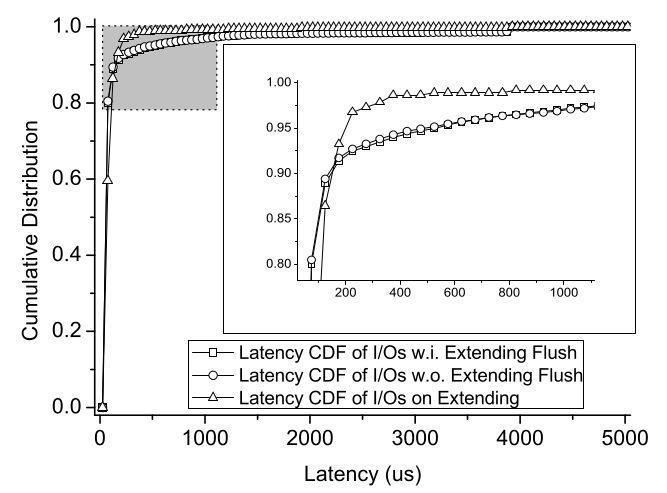
\includegraphics[width=0.8\textwidth]{translate_fig9.png}
    \caption*{图~9\hskip1em 扩展更新窗口的开销}
  \end{figure}

更新窗口用于减少系统崩溃后的扫描时间,但由于扩展更新窗口时存在索引持久性而导致额外写入。为了评估开销,我们收集了每个操作的I / O延迟的两个数据集,一个用于正常扩展,另一个用于没有索引持久性的扩展。两个数据集中潜伏期的累积分布用图9中几乎相同的线描绘,显示了接近的性能。我们还会在扩展期间识别I / O并收集每个I / O的延迟时间,以显示对外部I / O延迟的影响。扩展期间I / O的延迟与所有I / O的平均值相差不大。在该图的放大部分中,即使延迟I / O的累积分布在延迟小于200us时比平均增长慢,当延迟大约为200us时,其增长得更快。结果,扩展的I / O中有99.6%的延迟小于400us。此外,扩展操作很少出现,只有0.04%的I / O满足扩展。因此,我们得出结论:扩展更新窗口对性能的影响有限。

\section{相关工作}
Flash文件系统[32,10,9]利用闪存的nooverwrite属性进行日志结构更新,通过直接管理闪存来优化性能。但除了磨损平衡之外,他们对闪光耐力没有太大的贡献。无名写入[35]和直接文件系统[20]建议删除文件系统的映射,以允许FTL管理存储空间以提高性能。但是文件语义无法传递给FTL进行智能存储空间管理。 OFTL采用基于对象的存储的概念[25]将对象接口导出到文件系统,从而轻松地将文件语义传递到设备以进行智能数据布局。

最近的研究还提出消除闪存中日志造成的重复写入。 Write Atomic [28]通过利用FusionIO ioDrives中VSL [4]的基于日志的结构导出原子写入接口。 TxFlash [29]在页面元数据的帮助下使用循环提交协议来导出相同的接口。但是,循环属性维护起来很复杂,并且该协议在故障后需要进行全驱动扫描。相比之下,OFTL采用与日志结构文件系统[31]中的事务支持类似的简单协议,将事务信息保存在页面元数据中,并在更新窗口中跟踪最近更新的闪存块以便快速恢复。

在磁盘存储系统中使用反向指针来避免在Backlog中移动文件系统块时的文件系统元数据更新[24],或者通过将后向指针嵌入数据块,目录条目和Backpointerbased一致性中的inode来提供后续一致性检查[16] 。在基于闪存的存储中,LazyFTL [23]建议通过在页面元数据中保留逻辑页面编号(LPN)作为反向指针,并将页面记录在更新闪存块区域中,来懒惰地更新页面级FTL的映射条目,以块级FTL为代价提供页面级FTL的性能。但它不会触及文件系统中的元数据,这对写入放大作出了很大贡献。相反,OFTL利用页面元数据优化系统设计,并使用反向指针作为索引元数据惰性持久性的反向索引。

CAFTL [15]和DeltaFTL [33]合并冗余数据并压缩FTL中的相似页面,而LFS [13],JFFS2 [32],UBIFS [9]和btrfs [2]压缩文件中的数据页系统。他们都通过利用页面内容相似性来使用压缩,这与使用OFTL中访问大小信息的压缩更新技术正交。 IPL(页内记录)[22]采用类似于OFTL的方法,并在每个闪存块中保留一个日志区域以吸收小的更新。但是,如果数据和元数据页面分布在多个闪存块中,则会受到同步写入的影响。 reiserfs [7]中的尾部打包与OFTL中的压缩更新技术最相关。 Reiserfs将每个文件的尾部包装在其inode中。 OFTL与OFTL以不覆盖的方式更新不同,因此OFTL不仅压缩尾部,而且压缩每个写入操作的头部,包括追加和更新操作。

\section{结论}
传统文件系统专注于顺序存取优化,而不是写入放大缩小,这对闪存非常重要。系统机制(如日志记录,元数据同步和页面对齐更新)极大地放大了写入强度,而间接性带来的透明性阻止了系统利用闪存特性。在本文中,我们提出了一个基于对象的设计名称OFTL,其中存储管理从文件系统卸载到FTL以直接管理闪存。页面元数据用于保留延迟索引的反向索引和事务信息,以便为日志删除提供写入原子性,借助更新窗口跟踪尚未检查点的最新分配的闪存块。另外,空闲空间管理可以跟踪闪存块状态而不是页面状态,并降低状态持久化的频率以进一步降低元数据成本。使用字节单位访问接口,OFTL中标识的部分页面更新被压缩并与元数据共存以减少更新。在系统与闪存共同设计的情况下,文件系统的写入放大显著减少。

\section*{致谢}
我们要感谢我们的指导者Margo Seltzer和匿名审稿人提出的富有洞察力的意见和详细的建议,这大大改进了本文的内容和陈述。 我们也感谢Shuai Li在实验装置方面的帮助,Guangyu Sun在演讲中的帮助。 本研究由国家自然科学基金(批准号:60925006),国家自然科学基金重点项目(批准号:61232003),国家高技术研究发展计划(批准号: 2013AA013201),清华腾讯互联网创新技术联合实验室研究基金支持。

% \section*{参考文献}

% \begin{translationbib}
% \item blktrace(8) - linux man page. http://linux.die.net/man/8/blktrace.
% \item Btrfs. http://btrfs.wiki.kernel.org.
% \item Dbt2 test suite. http://sourceforge.net/apps/mediawiki/osdldbt.
% \item Fusionio virtual storage layer. http://www/fusionio.com/products/vsl.
% \item Lasr system call io trace. http://iotta.snia.org/tracetypes/1.
% \item The nvm express standard. http://www.nvmexpress.org.
% \item Reiserfs. http://reiser4.wiki.kernel.org.
% \item strace(1) - linux man page. http://linux.die.net/man/1/strace.
% \item Ubifs - ubi file-system. http://www.linux-mtd.infradead.org/doc/ubifs.html.
% \item Yaffs. http://www.yaffs.net.
% \item N. Agrawal, V. Prabhakaran, T. Wobber, J. D. Davis, M. Manasse, and R. Panigrahy. Design tradeoffs for ssd performance. In Proceedings of USENIX 2008 Annual Technical Conference, 2008.
% \item S. Boboila and P. Desnoyers. Write endurance in flash drives: measurements and analysis. In Proceedings of the 8th USENIX conference on File and storage technologies (FAST), 2010.
% \item Michael Burrows, Charles Jerian, Butler Lampson, and Timothy Mann. On-line data compression in a log-structured file system. In Proceedings of the fifth international conference on Architectural support for programming languages and operating systems (ASPLOS), 1992.
% \item L.P. Chang. On efficient wear leveling for large-scale flash-memory storage systems. In Proceedings of the 2007 ACM symposium on Applied computing, 2007.
% \item F. Chen, T. Luo, and X. Zhang. Caftl: A content-aware flash translation layer enhancing the lifespan of flash memory based solid state drives. In Proceedings of the 9th USENIX conference on File and Storage Technologies (FAST), 2011.
% \item V. Chidambaram, T. Sharma, A. C. Arpaci-Dusseau, and R. H. Arpaci-Dusseau. Consistency without ordering. In Proceedings of the 10th USENIX conference on File and Storage Technologies (FAST), 2012.
% \item L. M. Grupp, J. D. Davis, and S. Swanson. The bleak future of nand flash memory. In Proceedings of the 10th USENIX conference on File and Storage Technologies (FAST), 2012.
% \item L.M. Grupp, A.M. Caulfield, J. Coburn, S. Swanson, E. Yaakobi, P.H. Siegel, and J.K. Wolf. Characterizing flash memory: anomalies, observations, and applications. In Proceedings of the 42nd Annual IEEE/ACM International Symposium on Microarchitecture (MICRO-42), 2009.
% \item T. Harter, C. Dragga, M. Vaughn, A. C. Arpaci-Dusseau, and R. H. Arpaci-Dusseau. A file is not a file: understanding the i/o behavior of apple desktop applications. In Proceedings of the 23rd ACM Symposium on Operating Systems Principles (SOSP), 2011.
% \item W. K. Josephson, L. A. Bongo, D. Flynn, and K. Li. Dfs: a file system for virtualized flash storage. In Proceedings of the 8th USENIX conference on File and Storage Technologies (FAST), 2010.
% \item Y. Kang, J. Yang, and E. L. Miller. Object-based scm: An efficient interface for storage class memories. In Proceedings of IEEE 27th Symposium on Mass Storage Systems and Technologies (MSST), 2011.
% \item S. W. Lee and B. Moon. Design of flash-based dbms: an in-page logging approach. In Proceedings of the 2007 ACM SIGMOD International Conference on Management of Data (SIGMOD), 2007.
% \item D. Ma, J. Feng, and G. Li. Lazyftl: A page-level flash translation layer optimized for nand flash memory. In Proceedings of the 2011 International Conference on Management of Data (SIGMOD), 2011.
% \item P. Macko, M. Seltzer, and K.A. Smith. Tracking back references in a write-anywhere file system. In Proceedings of the 8th USENIX conference on File and storage technologies (FAST), 2010.
% \item M. Mesnier, G.R. Ganger, and E. Riedel. Object-based storage. IEEE Communications Magazine, 41(8):84–90, 2003.
% \item D. Nellans, M. Zappe, J. Axboe, and D. Flynn. ptrim ()+ exists (): Exposing new ftl primitives to applications. In 2nd Annual Non-Volatile Memory Workshop, 2011.
% \item P. O’Neil, E. Cheng, D. Gawlick, and E. O’Neil. The log-structured merge-tree (lsm-tree). Acta Informatica, 33(4):351–385, 1996.
% \item X. Ouyang, D. Nellans, R. Wipfel, D. Flynn, and D. K. Panda. Beyond block i/o: Rethinking traditional storage primitives. In Proceedings of the 17th IEEE International Symposium on High Performance Computer Architecture (HPCA), 2011.
% \item V. Prabhakaran, T. L. Rodeheffer, and L. Zhou. Transactional flash. In Proceedings of the 8th USENIX conference on Operating Systems Design and Implementation (OSDI), 2008.
% \item O. Rodeh, J. Bacik, and C. Mason. Btrfs: The linux b-tree filesystem. Technical report, IBM Almaden Reserach Center, 2012.
% \item M. Seltzer. Transaction support in a log-structured file system. In Proceedings of the Ninth International Conference on Data Engineering, 1993.
% \item David Woodhouse. Jffs2: The journalling flash file system, version 2. http://sourceware.org/jffs2.
% \item G. Wu and X. He. Delta-ftl: improving ssd lifetime via exploiting content locality. In Proceedings of the 7th ACM European Conference on Computer Systems (EuroSys), 2012.
% \item Q. Yang and J. Ren. I-cash: Intelligently coupled array of ssd and hdd. In Proceedings of the 17th IEEE International Symposium on High Performance Computer Architecture (HPCA), 2011.
% \item Y. Zhang, L. P. Arulraj, A. C. Arpaci-Dusseau, and R. H. Arpaci-Dusseau. De-indirection for flash-based ssds with nameless writes. In Proceedings of the 10th USENIX conference on File and Storage Technologies (FAST), 2012.
% \end{translationbib}

% \title{书面翻译对应的原文索引}
\begin{translationbib}
\item Lu Y, Shu J, ZhengW. Extending the Lifetime of Flash-based Storage through Reducing Write Amplication from File Systems[Z]. 14.
\end{translationbib}
